\section{Enabling Coverage/Overhead Trade-off}
\label{sec:drop}

Figure~\ref{dummy} shows the overheads of array bounds check with filtering
based on initialized metadata (see Section~\ref{sec:evaluation} for details on
the experimental methodology). The overheads range from XX\% to XX\%. In some
contexts, this overhead may still be considered to be too high. In this
section, we discuss how we can selectively perform monitoring in order to
further reduce overheads and match a specified overhead budget.

The high-level idea is to drop monitoring operations in order to remain within
the specified overhead budget. Given an overhead budget, the system estimates
the run-time overhead caused by monitoring (Section~\ref{sec:drop.slack}). When
this overhead exceeds the budget, then the system drops monitoring operations.
In order to prevent false positives, we must be able to identify flows that
have been dropped. This can be done by extending the dataflow engine to keep
track of an additional \emph{invalid flag} (Section~\ref{sec:drop.false_positives}). 

\subsection{Measuring Overheads}
\label{sec:drop.slack}

% Slack
\begin{figure}
  \begin{center}
    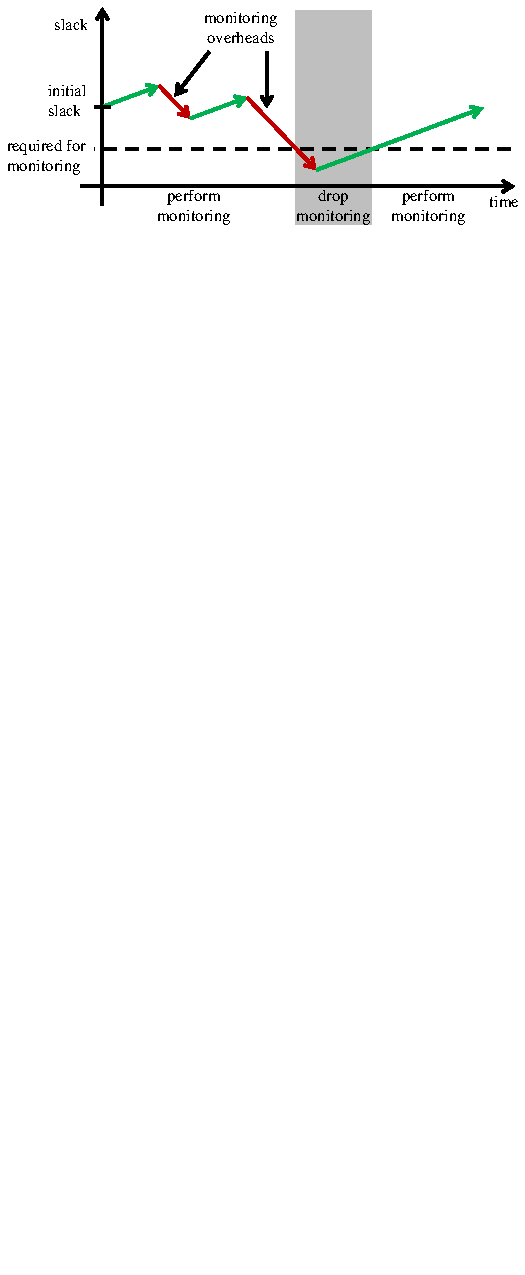
\includegraphics[width=\columnwidth]{figs/slack.pdf}
    \vspace{-0.3in}
    \caption{Slack and its effect on monitoring over time.}
    \label{fig:drop.slack}
    \vspace{-0.2in}
  \end{center}
\end{figure}

% Slack tracking module
\begin{figure}
  \begin{center}
    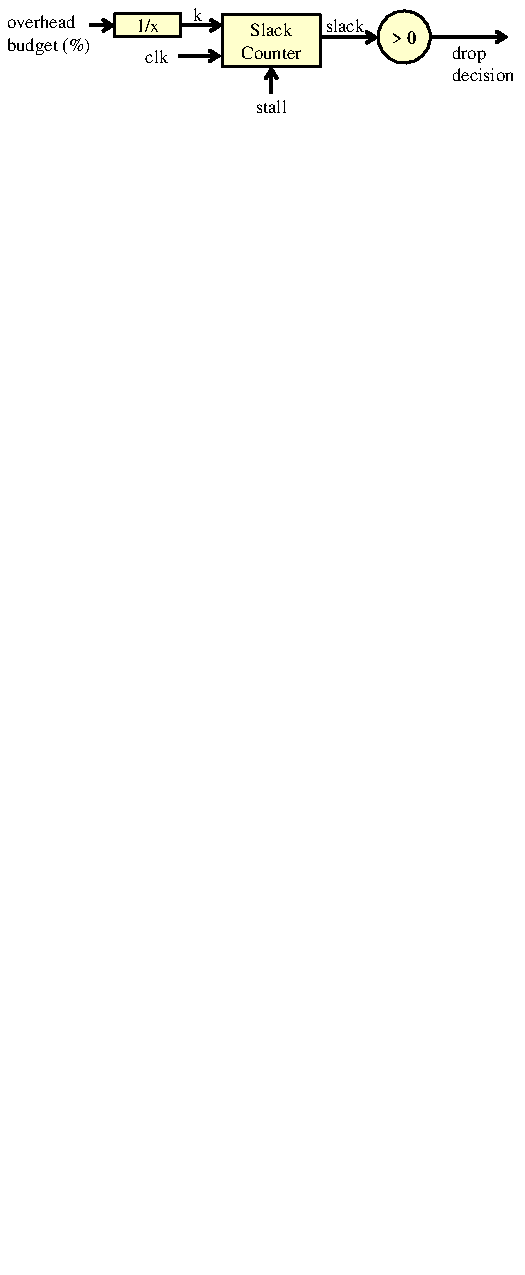
\includegraphics[width=\columnwidth]{figs/stm.pdf}
    \vspace{-0.3in}
    \caption{Slack tracking and drop decision hardware.}
    \label{fig:drop.stm}
    \vspace{-0.1in}
  \end{center}
\end{figure}

In order to decide whether a monitoring event should be dropped or not, we need
a way to keep track of overheads. In this section, we present a specific method
for measuring execution time overheads. However, we note that other methods
could be used in order to target budgets on IPC, power, energy, etc.  
% For example, one way to measure execution time overheads would be to insert
% checkpoints in the program. By recording the execution time of these
% checkpoints without monitoring, the overheads incurred while running with
% monitoring could be determined. Although this would give an accurate
% measurement of overheads, it would require modifying the program binary. In
% addition, the overhead budget for monitoring would only be updated at
% checkpoints.

% Instead, we develop a model to estimate the execution time overhead budget in a
% gradual manner and without the need to modify the main program. Specifically,
We specify the overhead budget as a percentage of the main program's execution
cycles without monitoring. We define \emph{slack} as the number of cycles of
monitoring overhead that can be incurred while staying within the budget
target. Slack is essentially the difference between the actual overheads seen
and the budget specified. Slack is generated as the main program runs.  For
example, if no monitoring overheads occur during 1000 cycles of the main
program's execution and the designer sets a 20\% overhead target, then the
slack that is built up during this period is 200 cycles. This slack can be used
to perform monitoring without exceeding the overhead budget.
Figure~\ref{fig:drop.slack} shows an example of how slack can change over time.
As monitoring overheads occur, the slack is decremented. 
% If the slack falls below the overhead expected for handling a monitoring event,
% then the event is dropped. 
If the slack falls below zero (i.e., the overhead budget is exceeded), then
monitoring events are dropped.
In addition to this accumulated slack, a small amount of initial slack
can be given in order for monitoring to be performed at the start of a program.

Figure~\ref{fig:drop.stm} shows a hardware slack tracking module (STM) for
keeping track of slack. The STM uses a counter that increments on every $k$-th
cycle of the main core. This $k$ can be calculated by taking the reciprocal of
the target budget. For example, if the target budget is 20\%, then the counter
increments on every 5th clock cycle. The value of this counter is the
accumulated slack. Whenever the main core is stalled due to the monitor, slack
is decremented.

% In addition to keeping track of overheads, a policy must be developed to
% determine when monitoring event should be dropped. Complex policies involving
% multiple conditions and safety factors could be used to finely tune
% the trade off between monitoring and performance overhead. Similarly, introducing
% randomness into the policy could allow for better sampling in a cooperative
% debugging application of monitoring. Here, we present one simple
% dropping policy that is based on the accumulated slack.
% When the monitor is initialized, the monitor will load
% its needed slack in order to perform a monitoring operation into a register. When
% there is a monitoring event in the FIFO to be processed, a hardware comparator
% checks whether the accumulated slack is greater than or equal to the necessary
% slack for full monitoring. If enough slack exists, the monitor is signaled to
% perform the monitoring operation. Otherwise, the monitoring event is dropped.

\subsection{Preventing False Positives}
\label{sec:drop.false_positives}

Dropping a monitoring operation implies that some functionality of the monitor
has been lost. This may cause either false negatives, where an error that
occurs in the main program's execution is not detected, or false positives,
where the monitor incorrectly believes an error has occurred. 
% For example, a
% false positive can occur for UMC if a store monitoring event is dropped. This
% causes the store memory location to not be marked as initialized. A subsequent
% load for the memory location will incorrectly cause an error to be raised.  
For example, a false positive can occur for array bounds check if an event is
dropped that handles copying a pointer. A subsequent array access using the new
pointer will incorrectly cause an error to be raised since the new pointer's
base and bounds will not be correctly set.
We
accept false negatives as the loss in coverage that we trade off in order to
limit overheads.  However, we must safely drop monitoring events in such a way
as to avoid false positives so that the system does not incorrectly raise an
error.

In analyzing various monitoring schemes, we found that monitoring operations
are primarily of two types: \emph{checks} and \emph{metadata updates}. Monitors
\emph{check} certain properties to ensure correct main program execution and
they \emph{update} metadata for bookkeeping. Skipping a check operation can
only cause false negatives and will never cause a false positive. Therefore, we
may simply skip a check operation. Skipping an update operation can cause false
negatives but may also cause false positives. Essentially, when an update
operation is skipped, we can no longer trust the corresponding metadata.  Thus,
by associating an invalid flag with each metadata we can mark metadata that is
not correctly updated and use this information to prevent false positives.

% Flag propagation rules for BC
\begin{table}[tb]
  \begin{center}
    \begin{small}
    
% Initalized/Invalid flag propagation rules for BC/DIFT

\begin{tabular}{|c||c|c|c|c||c|c|c|c|}
\hline

{\bf Instruction} & \multicolumn{4}{c|}{\bf Initialized (src0, src1)} & \multicolumn{4}{c|}{\bf Invalid (src0, src1)} \\ \cline{2-9}
{\bf Type} & {\bf 00} & {\bf 01} & {\bf 10} & {\bf 11} & {\bf 00} & {\bf 01} & {\bf 10} & {\bf 11} \\ \hline

{\tt load} & 0 & 0 & X & X & X & X & 1 & 1 \\ \hline
{\tt store} & 0 & 0 & X & X & X & X & 1 & 1 \\ \hline
{\tt ALU} & 0 & X & X & X & X & 1 & 1 & 1 \\ \hline

\end{tabular}

    \end{small}
    \caption{Flag propagation rules for array bounds check. X indicates that no
    propagation is done while 0 or 1 indicates that the destination flag is set
    to that value.}
    \label{tab:drop.propagation_rules}
    \vspace{-0.2in}
  \end{center}
\end{table}

We extend the dataflow engine to keep track of invalidation flags in addition
to the clean flags discussed in Section~\ref{sec:filter}.
Since metadata derived from dropped metadata is also invalid. We propagate the
drop flag in a similar manner to the clean flags.  In the typical case, the
propagation rule is
that if any of the source operands is marked as invalid, then the destination
operand is marked as dropped. This is slightly different than the
policy for clean flags which propagates a clean flag only if both
sources are marked as clean. Table~\ref{tab:drop.propagation_rules} shows the
propagation rules that we use for array bounds check.  However, we note that
the propagation rules can be customized depending on the monitor by
reconfiguring the Filter Decision Table.
Similarly to filtering for clean flags, we can also filter out
useless monitoring for invalid metadata.
Thus, we see that by tracking two bits of information, we are able to use the
dataflow engine to both filter out monitoring operations for clean metadata as
well as selectively perform monitoring without false positives.

\subsection{Dropping Decision}

% Varying slack's impact on coverage for UMC
\begin{figure}
  \begin{center}
    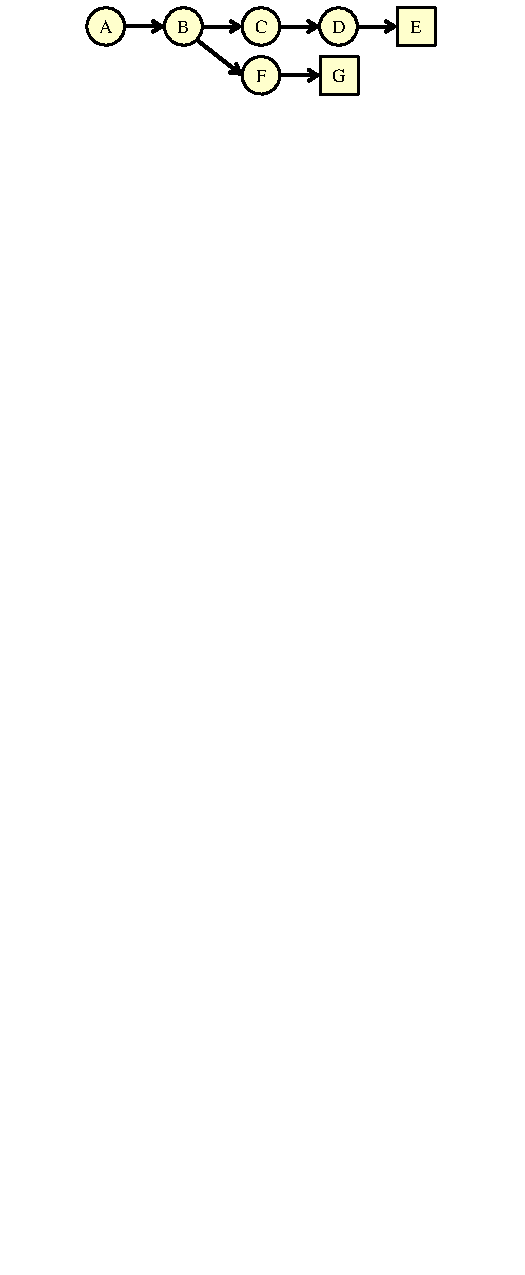
\includegraphics[width=\columnwidth]{figs/dataflow_graph.pdf}
    \vspace{-0.3in}
    \caption{Example dependence graph for metadata. Blue (dark) nodes represent
    events where checks are performed.}
    \label{fig:drop.dataflow_graph}
    \vspace{-0.1in}
  \end{center}
\end{figure}

One of the issues with waiting until the overhead budget is reached (i.e.,
slack is zero) to start dropping monitoring events is that this can result in
wasted work. For example, consider the metadata dependence graph shown in
Figure~\ref{fig:drop.dataflow_graph}. Here, an edge from node {\tt A} to node
{\tt B} represents that if event {\tt A} is dropped, then due to its
invalidated metadata, it will cause event {\tt B} to be also dropped. In the
example, we see that if event {\tt E} is dropped, then this meant that
monitoring for events {\tt C} and {\tt D} was wasted. The results of those
monitoring operations were not used for any monitoring checks.

One method to eliminate this wasted work is to only make dropping decisions at
the root of these metadata flow graphs. That is, we will decide to either monitor or
not monitor an entire metadata flow. We refer to this dropping decision policy
as \emph{source dropping} and we refer to the previous policy of waiting until
the overhead budget is reached as \emph{last-minute dropping}. Source dropping will
result in no wasted work. However, because of the coarser-grained decision, it
may be more difficult to closely match overheads. Source dropping is expected
to work well when there are a large number of independent metadata flows.

Another possible method is to make the dropping decisions somewhere in between
\emph{source dropping} and \emph{last-minute dropping}. From
Figure~\ref{fig:drop.dataflow_graph}, what we would like to do is make a
decision at event {\tt C} whether to perform monitoring on that branch of the
metadata flow. If we choose to perform monitoring, then we want to perform all
monitoring on that flow. Instead, if we choose to drop event {\tt C}, then the
entire flow is dropped with no wasted work. Similarly, dropping event {\tt F}
drops the bottom flow with no wasted work and event {\tt A} can be dropped to
drop the entire shown metadata flow with no wasted work. If the program can be
analyzed or profiled to identify these instructions which, if dropped, lead to
no wasted work, then this information can be used at run-time to minimize the
amount of wasted work. We refer to this policy as \emph{min-point dropping}.
Min-point dropping is a coarser-grained decision than last-minute dropping, but
finer-grained that source dropping. Thus, its ability to match overheads is
expected to sit between these other two policies. Similarly, there is still a
chance of wasted work due to strange splitting and merging metadata flow graph
shapes but typically we expect much less wasted work than last-minute
dropping. Thus, we expect the coverage achieved by min-point dropping for a
certain overhead to fall between source and last-minute dropping. These three
dropping policies create a trade-off space between coverage achieved and
ability to match an overhead target which we evaluate in detail in
Section~\ref{sec:evaluation}.

\subsection{Multiple-Run Coverage}
Coverage can be considered for a single or average run instance. It can also be
measured over multiple users/runs in order to capture total bug coverage of a
program.

The system presented so far operates in a deterministic manner and so each run
will perform the same monitoring checks. However, we can introduce randomness
in order to achieve different dropping patterns over runs and achieve higher
multiple-run coverage.

Due to the multiplicative effect of randomness, long dependence flows with
multiple points where randomness is introduced leads to a small chance that the
entire flow is monitored. This is a significant issue for last-minute dropping
where all events could be dropped. Min-point dropping reduces this effect by
reducing the points where dropping decisions are made while source-dropping
eliminates this issue entirely.

\subsection{Multi-Core Implementation}

This can be extended to mulit-core by using multiple dataflow engines and a
similar coherency protocol as that used for data caches.
